\documentclass[]{article}
\usepackage{lmodern}
\usepackage{amssymb,amsmath}
\usepackage{ifxetex,ifluatex}
\usepackage{fixltx2e} % provides \textsubscript
\ifnum 0\ifxetex 1\fi\ifluatex 1\fi=0 % if pdftex
  \usepackage[T1]{fontenc}
  \usepackage[utf8]{inputenc}
\else % if luatex or xelatex
  \ifxetex
    \usepackage{mathspec}
  \else
    \usepackage{fontspec}
  \fi
  \defaultfontfeatures{Ligatures=TeX,Scale=MatchLowercase}
\fi
% use upquote if available, for straight quotes in verbatim environments
\IfFileExists{upquote.sty}{\usepackage{upquote}}{}
% use microtype if available
\IfFileExists{microtype.sty}{%
\usepackage{microtype}
\UseMicrotypeSet[protrusion]{basicmath} % disable protrusion for tt fonts
}{}
\usepackage[margin=1in]{geometry}
\usepackage{hyperref}
\hypersetup{unicode=true,
            pdftitle={Managing for ecological surprises in metapopulations},
            pdfborder={0 0 0},
            breaklinks=true}
\urlstyle{same}  % don't use monospace font for urls
\usepackage{color}
\usepackage{fancyvrb}
\newcommand{\VerbBar}{|}
\newcommand{\VERB}{\Verb[commandchars=\\\{\}]}
\DefineVerbatimEnvironment{Highlighting}{Verbatim}{commandchars=\\\{\}}
% Add ',fontsize=\small' for more characters per line
\usepackage{framed}
\definecolor{shadecolor}{RGB}{248,248,248}
\newenvironment{Shaded}{\begin{snugshade}}{\end{snugshade}}
\newcommand{\AlertTok}[1]{\textcolor[rgb]{0.94,0.16,0.16}{#1}}
\newcommand{\AnnotationTok}[1]{\textcolor[rgb]{0.56,0.35,0.01}{\textbf{\textit{#1}}}}
\newcommand{\AttributeTok}[1]{\textcolor[rgb]{0.77,0.63,0.00}{#1}}
\newcommand{\BaseNTok}[1]{\textcolor[rgb]{0.00,0.00,0.81}{#1}}
\newcommand{\BuiltInTok}[1]{#1}
\newcommand{\CharTok}[1]{\textcolor[rgb]{0.31,0.60,0.02}{#1}}
\newcommand{\CommentTok}[1]{\textcolor[rgb]{0.56,0.35,0.01}{\textit{#1}}}
\newcommand{\CommentVarTok}[1]{\textcolor[rgb]{0.56,0.35,0.01}{\textbf{\textit{#1}}}}
\newcommand{\ConstantTok}[1]{\textcolor[rgb]{0.00,0.00,0.00}{#1}}
\newcommand{\ControlFlowTok}[1]{\textcolor[rgb]{0.13,0.29,0.53}{\textbf{#1}}}
\newcommand{\DataTypeTok}[1]{\textcolor[rgb]{0.13,0.29,0.53}{#1}}
\newcommand{\DecValTok}[1]{\textcolor[rgb]{0.00,0.00,0.81}{#1}}
\newcommand{\DocumentationTok}[1]{\textcolor[rgb]{0.56,0.35,0.01}{\textbf{\textit{#1}}}}
\newcommand{\ErrorTok}[1]{\textcolor[rgb]{0.64,0.00,0.00}{\textbf{#1}}}
\newcommand{\ExtensionTok}[1]{#1}
\newcommand{\FloatTok}[1]{\textcolor[rgb]{0.00,0.00,0.81}{#1}}
\newcommand{\FunctionTok}[1]{\textcolor[rgb]{0.00,0.00,0.00}{#1}}
\newcommand{\ImportTok}[1]{#1}
\newcommand{\InformationTok}[1]{\textcolor[rgb]{0.56,0.35,0.01}{\textbf{\textit{#1}}}}
\newcommand{\KeywordTok}[1]{\textcolor[rgb]{0.13,0.29,0.53}{\textbf{#1}}}
\newcommand{\NormalTok}[1]{#1}
\newcommand{\OperatorTok}[1]{\textcolor[rgb]{0.81,0.36,0.00}{\textbf{#1}}}
\newcommand{\OtherTok}[1]{\textcolor[rgb]{0.56,0.35,0.01}{#1}}
\newcommand{\PreprocessorTok}[1]{\textcolor[rgb]{0.56,0.35,0.01}{\textit{#1}}}
\newcommand{\RegionMarkerTok}[1]{#1}
\newcommand{\SpecialCharTok}[1]{\textcolor[rgb]{0.00,0.00,0.00}{#1}}
\newcommand{\SpecialStringTok}[1]{\textcolor[rgb]{0.31,0.60,0.02}{#1}}
\newcommand{\StringTok}[1]{\textcolor[rgb]{0.31,0.60,0.02}{#1}}
\newcommand{\VariableTok}[1]{\textcolor[rgb]{0.00,0.00,0.00}{#1}}
\newcommand{\VerbatimStringTok}[1]{\textcolor[rgb]{0.31,0.60,0.02}{#1}}
\newcommand{\WarningTok}[1]{\textcolor[rgb]{0.56,0.35,0.01}{\textbf{\textit{#1}}}}
\usepackage{graphicx,grffile}
\makeatletter
\def\maxwidth{\ifdim\Gin@nat@width>\linewidth\linewidth\else\Gin@nat@width\fi}
\def\maxheight{\ifdim\Gin@nat@height>\textheight\textheight\else\Gin@nat@height\fi}
\makeatother
% Scale images if necessary, so that they will not overflow the page
% margins by default, and it is still possible to overwrite the defaults
% using explicit options in \includegraphics[width, height, ...]{}
\setkeys{Gin}{width=\maxwidth,height=\maxheight,keepaspectratio}
\IfFileExists{parskip.sty}{%
\usepackage{parskip}
}{% else
\setlength{\parindent}{0pt}
\setlength{\parskip}{6pt plus 2pt minus 1pt}
}
\setlength{\emergencystretch}{3em}  % prevent overfull lines
\providecommand{\tightlist}{%
  \setlength{\itemsep}{0pt}\setlength{\parskip}{0pt}}
\setcounter{secnumdepth}{0}
% Redefines (sub)paragraphs to behave more like sections
\ifx\paragraph\undefined\else
\let\oldparagraph\paragraph
\renewcommand{\paragraph}[1]{\oldparagraph{#1}\mbox{}}
\fi
\ifx\subparagraph\undefined\else
\let\oldsubparagraph\subparagraph
\renewcommand{\subparagraph}[1]{\oldsubparagraph{#1}\mbox{}}
\fi

%%% Use protect on footnotes to avoid problems with footnotes in titles
\let\rmarkdownfootnote\footnote%
\def\footnote{\protect\rmarkdownfootnote}

%%% Change title format to be more compact
\usepackage{titling}

% Create subtitle command for use in maketitle
\providecommand{\subtitle}[1]{
  \posttitle{
    \begin{center}\large#1\end{center}
    }
}

\setlength{\droptitle}{-2em}

  \title{Managing for ecological surprises in metapopulations}
    \pretitle{\vspace{\droptitle}\centering\huge}
  \posttitle{\par}
  \subtitle{Supplemental materials}
  \author{Kyle Logan Wilson\(^1\), Colin Bailey\(^1\), William Atlas\(^1\), and
Doug Braun\(^2\)\\
~\\
\(^1\)Earth to Ocean Research Group, Simon Fraser University\\
\(^2\)Fisheries \& Oceans Canada}
    \preauthor{\centering\large\emph}
  \postauthor{\par}
      \predate{\centering\large\emph}
  \postdate{\par}
    \date{30 May 2019}

\usepackage{wrapfig}
\usepackage{lipsum}
\usepackage{float}

\begin{document}
\maketitle

\hypertarget{metapopulation-model}{%
\subsection{Metapopulation model}\label{metapopulation-model}}

\hypertarget{local-metapopulation-dynamics}{%
\subsubsection{Local \& metapopulation
dynamics}\label{local-metapopulation-dynamics}}

Our metapopulation is defined by a set of local populations \(N_p\) with
time-dynamics that follows birth (i.e., recruitment \emph{R}),
immigration, death, and emigration (BIDE) processes:

\(N_{it}= R_{it}\epsilon_{it}+I_{it}-D_{it}-E_{it}\)

where \(N_{it+1}\) is the number of adults in patch \emph{i} at time
\emph{t}, \(R_{it}\) is number of recruits, \(I_{it}\) is number of
recruits immigrating into patch \emph{i} from any other patch,
\(D_{it}\) is number of recruits that die due to disturbance regime,
\(E_{it}\) is the number of recruits emigrating from patch \emph{i} into
any other patch, and \(\epsilon_{it}\) is stochasticity in recruitment.

Resoure monitoring often occurs at the scale of the metapopulation,
hence we define metapopulation adults as:

\({MN}_t = \sum_{i=1}^{N_p} N_{it}\)

with metapopulation recruits:

\(MR_t = \sum_{i=1}^{N_p} R_{it}\)

Local patch recruitment at time \emph{t} depended on adult densities at
\emph{t-1} and followed a reparameterized Beverton-Holt function:

\(R_{it}=\cfrac{\alpha_iN_{it-1}}{1+\cfrac{\alpha_i-1}{\beta_i}N_{it-1}}\)

where \(\alpha_i\) is the recruitment compensation ratio and \(\beta_i\)
is local patch carrying capacity.

For example, in a two patch model that varies \(\alpha_i\) and
\(\beta_i\) parameters such that

\begin{Shaded}
\begin{Highlighting}[]
\NormalTok{alpha <-}\StringTok{ }\KeywordTok{c}\NormalTok{(}\DecValTok{2}\NormalTok{, }\DecValTok{4}\NormalTok{)}
\NormalTok{beta <-}\StringTok{ }\KeywordTok{c}\NormalTok{(}\DecValTok{100}\NormalTok{, }\DecValTok{200}\NormalTok{)}
\end{Highlighting}
\end{Shaded}

Management often monitors metapopulation resources as the aggregate of
all local populations. In this way, recruitment compensation from local
patches \(\alpha_i\) gets averaged across the metapopulation leading
mean compensation \(\bar{\alpha}\) of 3. Likewise, the total carrying
capacity of the metapopulation \(\bar{\beta}\) becomes the summation of
local patch carrying capacities \(\sum\beta_i\), which is 300. This
scale of monitoring generates the following local patch and
metapopulation dynamics:

\begin{figure}[H]

{\centering 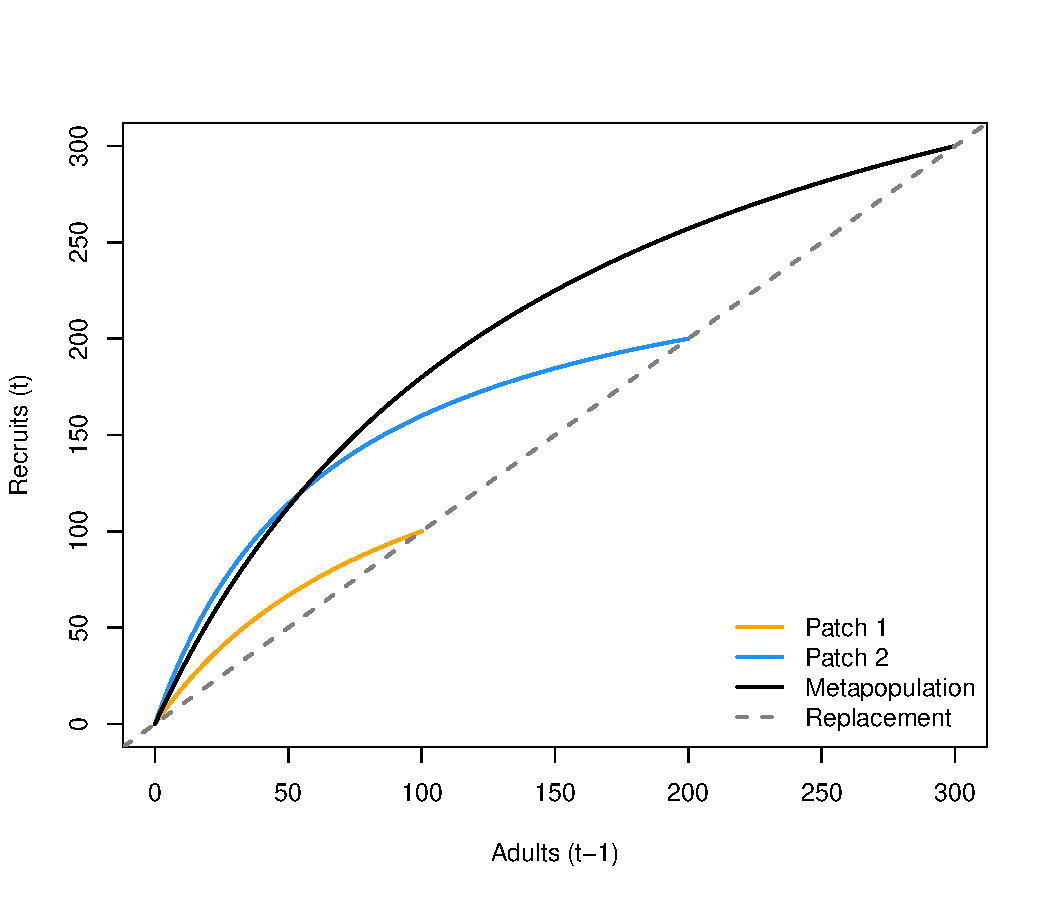
\includegraphics{Managing_for_ecological_surprises_in_metapopulations_makeHTML_files/figure-latex/recruit curves-1} 

}

\caption{Metapopulation and local patch recruitment dynamics.}\label{fig:recruit curves}
\end{figure}

\hypertarget{creating-the-spatial-networks}{%
\subsubsection{Creating the spatial
networks}\label{creating-the-spatial-networks}}

The next aspect to our metapopulation model is connecting the set of
patches to one another. We need to specify the number of patches, their
arrangements (i.e., connections), and how far apart they are from one
another. We followed some classic metapopulation and source-sink
arrangements to create four networks that generalize across a few
real-world topologies: a linear habitat network (e.g., coastline), a
dendritic or branching network (e.g., coastal rivers), a star network
(e.g., mountain \& valley), and a complex network (e.g., terrestrial
plants).

To make networks comparable, each spatial network type needs the same
leading parameters (e.g., \(N_p\) and \(\bar{d}\)) . In this case for
number of patches, we set \(N_p\) to \texttt{16} and \(\bar{d}\) to
\texttt{1} unit (distance units are arbitrary). We used the
\texttt{igraph} package and some custom code to arrange our spatial
networks as the following:

\begin{figure}[H]

{\centering 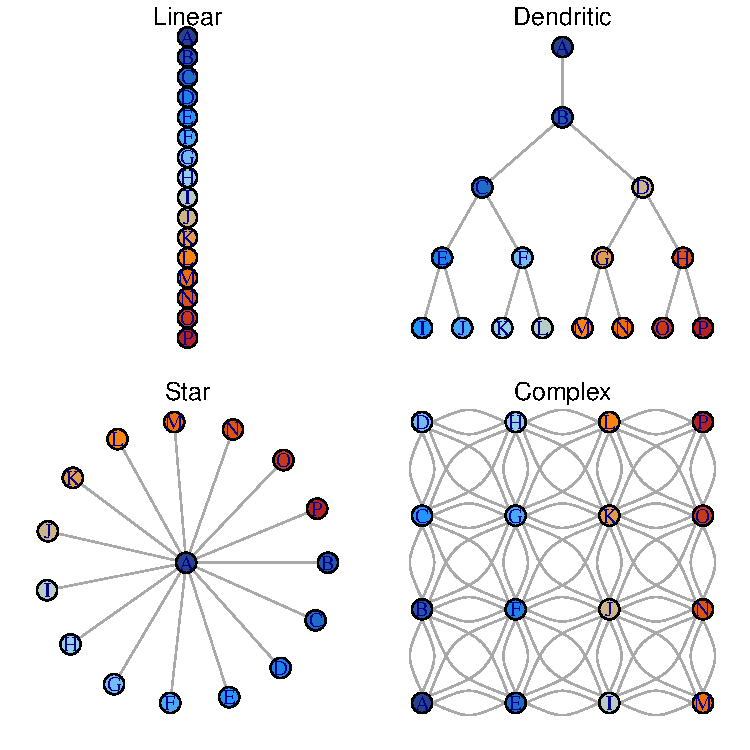
\includegraphics{Managing_for_ecological_surprises_in_metapopulations_makeHTML_files/figure-latex/networks-1} 

}

\caption{Four spatial network topologies.}\label{fig:networks}
\end{figure}

Note that distances between neighbor patches in the above networks are
equal.

An example dispersal matrix for the complex network:

\begin{verbatim}
##   A B E F C G D H I J K L M N O P
## A 0 1 1 1 2 2 3 3 2 2 2 3 3 3 3 3
## B 1 0 1 1 1 1 2 2 2 2 2 2 3 3 3 3
## E 1 1 0 1 2 2 3 3 1 1 2 3 2 2 2 3
## F 1 1 1 0 1 1 2 2 1 1 1 2 2 2 2 2
## C 2 1 2 1 0 1 1 1 2 2 2 2 3 3 3 3
## G 2 1 2 1 1 0 1 1 2 1 1 1 2 2 2 2
## D 3 2 3 2 1 1 0 1 3 2 2 2 3 3 3 3
## H 3 2 3 2 1 1 1 0 3 2 1 1 3 2 2 2
## I 2 2 1 1 2 2 3 3 0 1 2 3 1 1 2 3
## J 2 2 1 1 2 1 2 2 1 0 1 2 1 1 1 2
## K 2 2 2 1 2 1 2 1 2 1 0 1 2 1 1 1
## L 3 2 3 2 2 1 2 1 3 2 1 0 3 2 1 1
## M 3 3 2 2 3 2 3 3 1 1 2 3 0 1 2 3
## N 3 3 2 2 3 2 3 2 1 1 1 2 1 0 1 2
## O 3 3 2 2 3 2 3 2 2 1 1 1 2 1 0 1
## P 3 3 3 2 3 2 3 2 3 2 1 1 3 2 1 0
\end{verbatim}

\hypertarget{dispersal}{%
\subsubsection{Dispersal}\label{dispersal}}

Dispersal from patch \emph{i} into patch \emph{j} depends on constant
dispersal rate \(\omega\) (defined as the proportion of total local
recruits that will disperse) and an exponential distance-decay function
between \emph{i} and \emph{j} with distance cost to dispersal \(m\)
following:

\(E_{ij(t)}=\omega R_{it}p_{ij}\)

where \(E_{ij}\) is the total dispersing animals from patch \emph{i}
into patch \emph{j} and probability of dispersal between patches
\(p_{ij}\):

\(p_{ij}=\dfrac{e^{-md_{ij}}}{\sum\limits_{\substack{j=1 \\ j\neq i}}^{N_p} e^{-md_{ij}}}\)

where \(d_{ij}\) is the pairwise distance between patches. The summation
term in the denominator normalizes the probability of moving to any
patch to between 0 and 1. With \(\bar{d}= 1\), \(m=0.5\),
\(\omega=0.1\), \(R_{it}=100\) in a linear network:

\begin{figure}[H]

{\centering 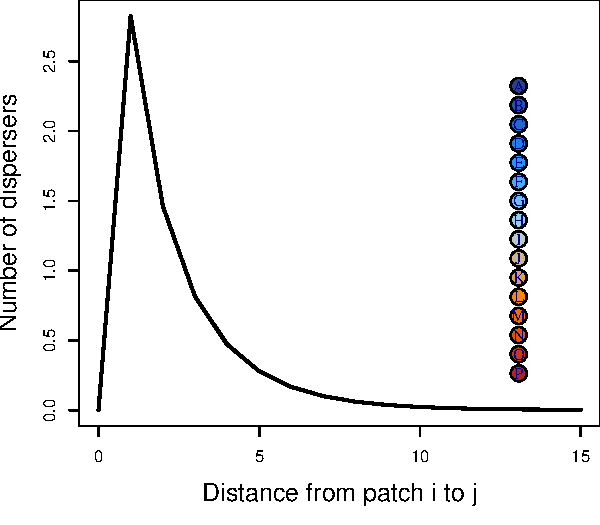
\includegraphics{Managing_for_ecological_surprises_in_metapopulations_makeHTML_files/figure-latex/dispersal-1} 

}

\caption{Example dispersal patterns across linear network.}\label{fig:dispersal}
\end{figure}

\hypertarget{recruitment-stochasticity}{%
\subsubsection{Recruitment
stochasticity}\label{recruitment-stochasticity}}

Enter some text here

\hypertarget{spatio-temporal-correlations}{%
\paragraph{Spatio-temporal
correlations}\label{spatio-temporal-correlations}}

Enter some more text here

\hypertarget{disturbance-regimes}{%
\subsubsection{Disturbance regimes}\label{disturbance-regimes}}

In all scenarios, disturbance was applied after \texttt{50} years of
equilibrating the metapopulaton at pristine conditions. At year
\texttt{50+1}, we applied the disturbance regime (the regime varied from
\emph{uniform}, \emph{localized, random}, and \emph{localized,
extirpation} - see \emph{Scenarios} below). Disturbance immediately
removes a set proportion of the metapopulation adults at that time
(i.e., \texttt{0.9} of \(MN_{t=51}\)). Once applied, the metapopulation
is no longer disturbed and spatio-temporal dynamics emerge naturally
from these new conditions.

\hypertarget{emergent-outcomes}{%
\subsection{Emergent outcomes}\label{emergent-outcomes}}

We measured the following ecological outcomes that have direction
application for conservation metrics.

\begin{enumerate}
\def\labelenumi{\arabic{enumi}.}
\item
  Recovered \& recovery rate after disturbance - the number of
  simulations where metapopulation abundance averaged \texttt{1.0}
  carrying capacity for \texttt{5} consecutive years post-disturbance
  and the number of years it took to get there.
\item
  Extinction \& extinction rate - the number of simulations where
  metapopulation abundance was \texttt{\textless{}0.05} carrying
  capacity and the mean number of years it took to get there.
\item
  Patch occupancy - the mean number of patches with
  \texttt{\textgreater{}0.1} local carrying capacity.
\item
  Spatial variance
\item
  Temporal variation in source, sink, pseudo-sink defined as:

  \begin{enumerate}
  \def\labelenumii{\alph{enumii}.}
  \tightlist
  \item
    Sources provide surplus recruits and net emigrants such that:
    \((R_{it}>N_{it})\) \& \((E_{it}>I_{it})\)
  \item
    Sinks consume recruits and net immigrants such that:
    \((R_{it} < N_{it})\) \& \((E_{it} < I_{it})\)
  \item
    Pseudo-sinks would provide surplus recruits in the absence of
    dispersal such that \((R_{it}>N_{it})\) but
    \((R_{it}+E_{it}) < (R_{it-1}+I_{it-1}-E_{it-1})\)
  \end{enumerate}
\item
  Fit stock-recruitment model to aggregate of metapopulation to
  estimate:

  \begin{enumerate}
  \def\labelenumii{\alph{enumii}.}
  \tightlist
  \item
    Recruitment compensaton ratio compared to true metapopulation
    average
  \item
    Metapopulation carrying capacities compared to true sum of carrying
    capacities across metapopulation
  \item
    Expected recruitment production to true recruitment production
    across all patches
  \item
    Expected maximum sustainable yield \emph{MSY} to true maximum
    sustainable yield across all patches
  \end{enumerate}
\end{enumerate}

\hypertarget{monitoring-management-at-aggregate-scale}{%
\subsubsection{Monitoring \& management at
aggregate-scale}\label{monitoring-management-at-aggregate-scale}}

While true metapopulation dynamics are controlled by local patch
dynamics and dispersal such that:

\(N_{it}= R_{it}\epsilon_{it}+I_{it}-D_{it}-E_{it}\)

\(R_{it}=\cfrac{\alpha_iN_{it-1}}{1+\cfrac{\alpha_i-1}{\beta_i}N_{it-1}}\)

\({MN}_t = \sum_{i=1}^{N_p} N_{it}\)

\({MR}_t = \sum_{i=1}^{N_p} R_{it}\)

natural resoure managers often monitors and manages at the scale of the
metapopulation. Hence, management at this scale inherently defines the
stock-recruitment dynamics of the aggregate complex of patches (i.e.,
metapopulation) as:

\({MR}_{t}=\cfrac{\hat{\alpha_t}{MN}_{t-1}}{1+\cfrac{\hat{\alpha_t}-1}{\hat{\beta_t}}{MN}_{it-1}}\)

where \(\hat{\alpha_t}\) is the estimated compensation ratio averaged
across the metapopulation at time \emph{t} and \(\hat{\beta_t}\) is the
estimated carrying capacity of the entire metapopulation. Necessarily,
these estimates emerge from monitoring data collected across all patches
and are sensitive to the quality of the data and how local patches
perform through time. For example, temporal shifts in productivity
regimes may be masked if most of the data were sampled before the regime
shift. To help surmount these issues, modern resource assessments use
data weighting and penalties (i.e., priors) when fitting models to data.

In our assessment, we weighted recent years of sampling over more
distant years such that:

\begin{figure}[H]

{\centering 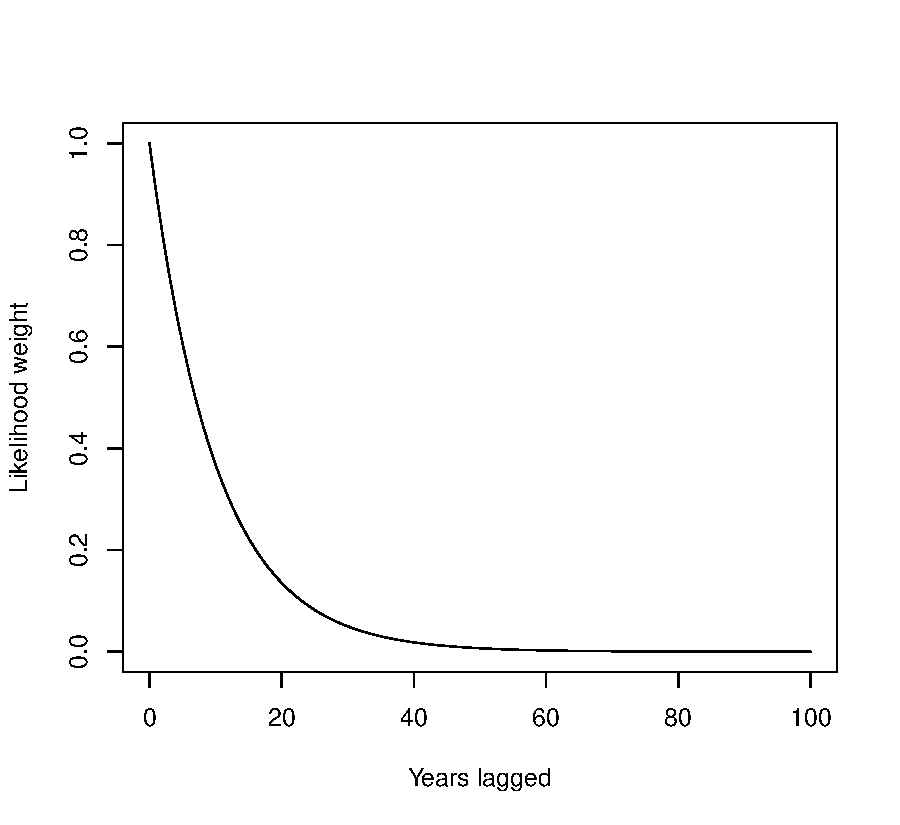
\includegraphics{Managing_for_ecological_surprises_in_metapopulations_makeHTML_files/figure-latex/unnamed-chunk-1-1} 

}

\caption{Likelihood weighting for samples collected over time from current year of sampling.}\label{fig:unnamed-chunk-1}
\end{figure}

Furthermore, we used penalized normal likelihoods on both
\(\hat{\alpha_t}\) and \(\hat{\beta_t}\) such that:

\(\hat{\alpha_t} \sim N(\mu=\hat{\alpha_{t-1}},\sigma=3\hat{\alpha_{t-1}})\)

and

\(\hat{\beta_t} \sim N(\mu=\hat{\beta_{t-1}},\sigma=3\hat{\beta_{t-1}})\)

where \(\mu=\hat{\alpha_{t-1}}\) and \(\mu=\hat{\beta_{t-1}}\)
represents the best estimates from the previous assessment and the
\texttt{3} in the \(\sigma\) term represents a 300\% coefficient of
variation. We used these penalized likelihoods to fit the above
aggregate stock-recruitment model with \emph{lognormal} error to the
metapopulation stock-recruit data collected at time \emph{t}. We used
the following function and fitted to the below \(\theta\) parameters
(termed \texttt{theta} in the function \texttt{optim()} using the
\texttt{L-BFGS-B} optimizer with a lower bound on \(\hat{\alpha}\) of
\texttt{1.01} (i.e., constrained to be at least above replacement).

\begin{Shaded}
\begin{Highlighting}[]
\NormalTok{SRfn <-}\StringTok{ }\ControlFlowTok{function}\NormalTok{(theta) \{}
\NormalTok{    a.hat <-}\StringTok{ }\NormalTok{theta[}\DecValTok{1}\NormalTok{]}
\NormalTok{    b.hat <-}\StringTok{ }\KeywordTok{exp}\NormalTok{(theta[}\DecValTok{2}\NormalTok{])}
\NormalTok{    sd.hat <-}\StringTok{ }\KeywordTok{exp}\NormalTok{(theta[}\DecValTok{3}\NormalTok{])}
\NormalTok{    rec.mean <-}\StringTok{ }\NormalTok{(a.hat }\OperatorTok{*}\StringTok{ }\NormalTok{spawnRec}\OperatorTok{$}\NormalTok{spawners)}\OperatorTok{/}\NormalTok{(}\DecValTok{1} \OperatorTok{+}\StringTok{ }\NormalTok{((a.hat }\OperatorTok{-}\StringTok{ }\DecValTok{1}\NormalTok{)}\OperatorTok{/}\NormalTok{b.hat) }\OperatorTok{*}\StringTok{ }\NormalTok{spawnRec}\OperatorTok{$}\NormalTok{spawners)}
    \CommentTok{# negative log likelihood on recruitment parameters}
\NormalTok{    nll <-}\StringTok{ }\DecValTok{-1} \OperatorTok{*}\StringTok{ }\KeywordTok{sum}\NormalTok{(}\KeywordTok{dlnorm}\NormalTok{(spawnRec}\OperatorTok{$}\NormalTok{recruits, }\DataTypeTok{meanlog =} \KeywordTok{log}\NormalTok{(rec.mean), }\DataTypeTok{sdlog =}\NormalTok{ sd.hat, }
        \DataTypeTok{log =} \OtherTok{TRUE}\NormalTok{) }\OperatorTok{*}\StringTok{ }\NormalTok{spawnRec}\OperatorTok{$}\NormalTok{weights, }\DataTypeTok{na.rm =} \OtherTok{TRUE}\NormalTok{)}
    \CommentTok{# penalized likelihood on estimated alpha}
\NormalTok{    penalty1 <-}\StringTok{ }\OperatorTok{-}\KeywordTok{dnorm}\NormalTok{(a.hat, alphaLstYr, }\DecValTok{3} \OperatorTok{*}\StringTok{ }\NormalTok{alphaLstYr, }\DataTypeTok{log =} \OtherTok{TRUE}\NormalTok{)}
    \CommentTok{# penalized likelihood on estimated carrying capacity}
\NormalTok{    penalty2 <-}\StringTok{ }\OperatorTok{-}\KeywordTok{dnorm}\NormalTok{(b.hat, metaKLstYr, }\DecValTok{3} \OperatorTok{*}\StringTok{ }\NormalTok{metaKLstYr, }\DataTypeTok{log =} \OtherTok{TRUE}\NormalTok{)}
\NormalTok{    jnll <-}\StringTok{ }\KeywordTok{sum}\NormalTok{(}\KeywordTok{c}\NormalTok{(nll, penalty1, penalty2), }\DataTypeTok{na.rm =} \OtherTok{TRUE}\NormalTok{)}
    \KeywordTok{return}\NormalTok{(jnll)}
\NormalTok{\}}
\end{Highlighting}
\end{Shaded}

This above function allows us to assess the bias in \(\hat{\alpha_t}\),
\(\hat{\beta_t}\), and \(\hat{MR_t}\) compared to true \(\bar{\alpha}\),
\(\bar{\beta}\), and \({MR}_t\) across the metapopulation. This then
allows us to see how much information management \& monitoring programs
are missing when they assess metapopulations at the aggregate (rather
than local) scales.

\hypertarget{finding-maximum-sustainable-yield-msy}{%
\subsubsection{Finding maximum sustainable yield
(MSY)}\label{finding-maximum-sustainable-yield-msy}}

Enter some more text here.

\hypertarget{scenarios}{%
\subsection{Scenarios}\label{scenarios}}

We tested all combinations of the following eight proccesses (below) and
ran a \texttt{100} bootstraps per scenario to estimate the mean for each
of the above outcomes.

\begin{enumerate}
\def\labelenumi{\arabic{enumi}.}
\item
  Homogenous and spatially variable recruitment compensation ratio
  across patches, i.e.~intrinsic rate of population growth
  (\(\alpha_i\)).
\item
  Homogenous and spatially variable local carrying capacity across
  patches, i.e.~asymptote of expected recruits at high adult densities
  (\(\beta_i\))
\item
  Disturbances where a proportion of individuals removed from
  metapopulation (e.g., \texttt{0.90}) occurs.

  \begin{enumerate}
  \def\labelenumii{\alph{enumii}.}
  \tightlist
  \item
    \emph{uniform} - random individuals removed at equal vulnerability
    across all patches.
  \item
    \emph{localized, random} - random individuals removed from randomly
    selected subset of patches (as long as target loss can be achieved
    in subset)
  \item
    \emph{localized, extirpation} - total extirpation of randomly
    selected subset of patches (as long as target loss can be achieved
    in subset)
  \end{enumerate}
\item
  Density-independent dispersal rates \(\omega\) from 0 to 20\% of
  individuals within a patch will disperse.
\item
  Topology of the spatial networks with linear, dendritic, star, and
  complex networks. Each network with \(N_p\) of \texttt{16} and
  distance between patches \(\bar{d}\) of \texttt{1}.
\item
  Stochastic recruitment deviates from low, medium, high coefficient of
  variation on lognormal error. Generate stochasticity in time-dynamics
  via random recruitement deviates away from expected.
\item
  Temporal correlation in recruitment deviates from low, medium, high
  correlation (i.e., good year at time \emph{t} begets good year at time
  \emph{t+1}).
\item
  Spatial correlation in recruitment deviates among patches from low,
  medium, to high correlation (i.e., neighboring patches go up or down
  together).
\end{enumerate}

\hypertarget{example-results}{%
\subsubsection{Example results}\label{example-results}}

We can demonstrate our concepts with a model on a linear network
composed of \texttt{16} patches, a dispersal rate of \texttt{0.01} and a
high enough dispersal cost such that individuals are willing to move
only to their closest neighboring patches. This limits the strength of
potential rescue effects. For this example, patches varied in their
productivity and carrying capacity but will have deterministic
population dynamics.

\begin{figure}[H]

{\centering 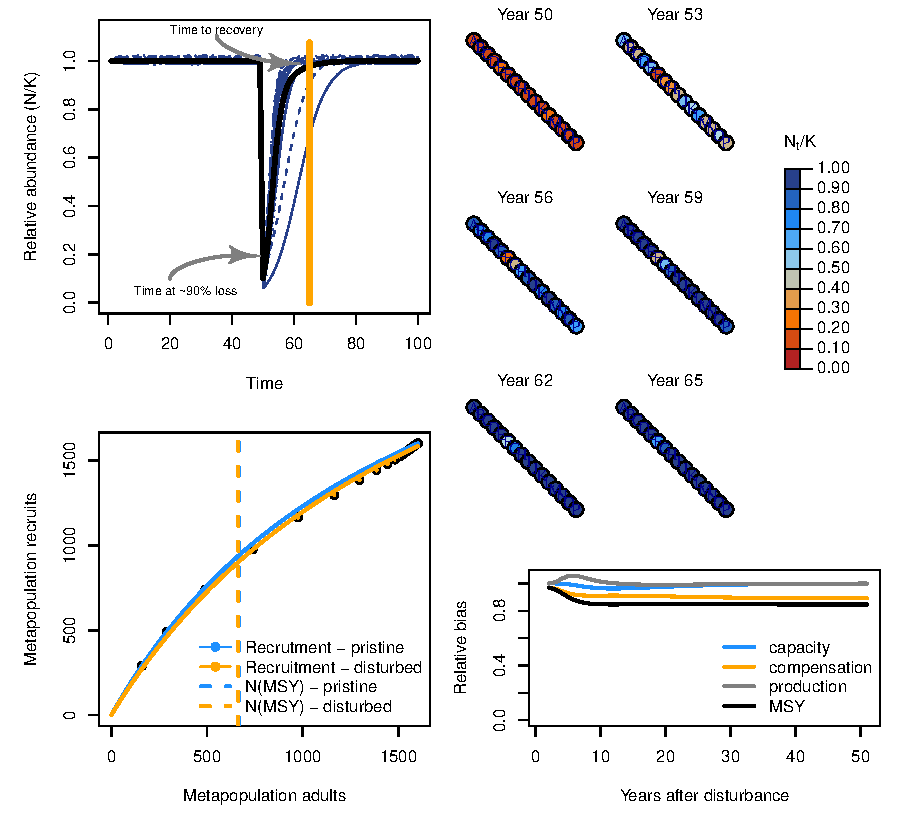
\includegraphics{Managing_for_ecological_surprises_in_metapopulations_makeHTML_files/figure-latex/example results1-1} 

}

\caption{Spatial recovery regime of metapopulation with linear topology through time (top left) and space (top right). Recruitment dynamics before and 10 years after disturbance (bottom left). Relative bias in aggregate-scale estimates of carrying capacity, compensation ratio, and recruitment production in recovery phase (bottom right).}\label{fig:example results1}
\end{figure}

We can then contrast this with a different network shape, like a
dendritic network.

\begin{figure}[H]

{\centering 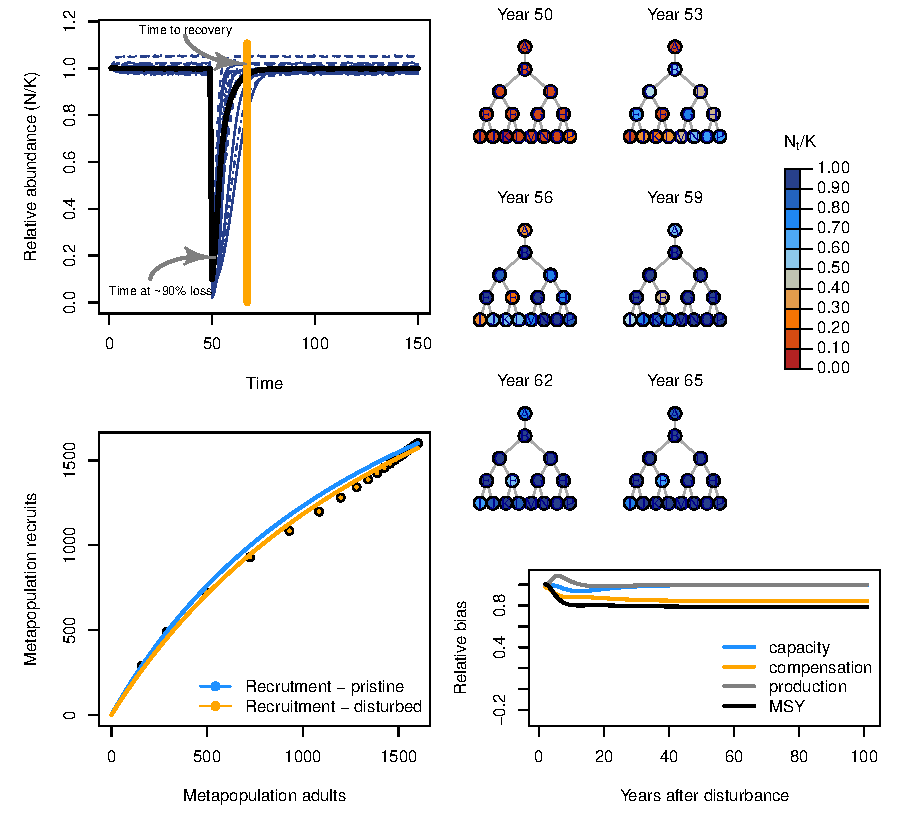
\includegraphics{Managing_for_ecological_surprises_in_metapopulations_makeHTML_files/figure-latex/example results2-1} 

}

\caption{Spatial recovery regime of metapopulation with dendritic topology.}\label{fig:example results2}
\end{figure}

Now, let's add some stochasticity to recruitment and see how this
affects the recovery regime.

\begin{figure}[H]

{\centering 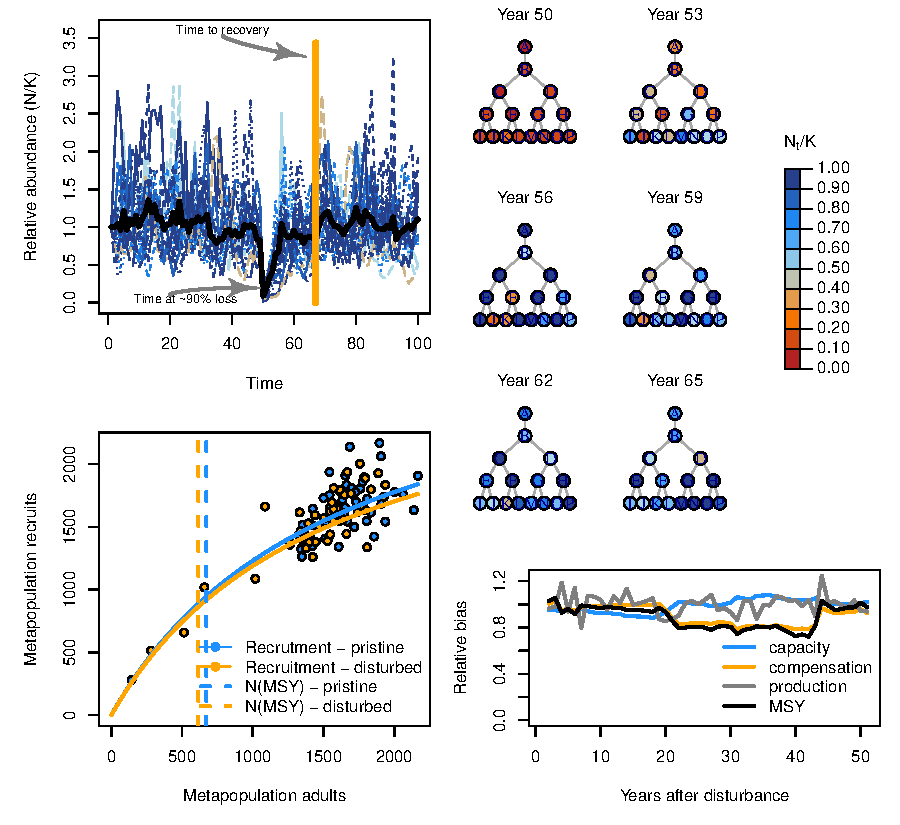
\includegraphics{Managing_for_ecological_surprises_in_metapopulations_makeHTML_files/figure-latex/example results3-1} 

}

\caption{Spatial recovery regime of stochastic metapopulation.}\label{fig:example results3}
\end{figure}

Next, we can contrast with a disturbance regime where the disturbance is
concentrated on local patches that can be completely extirpated (rather
than the disturbance being applied proportionally across all patches).

\begin{figure}[H]

{\centering 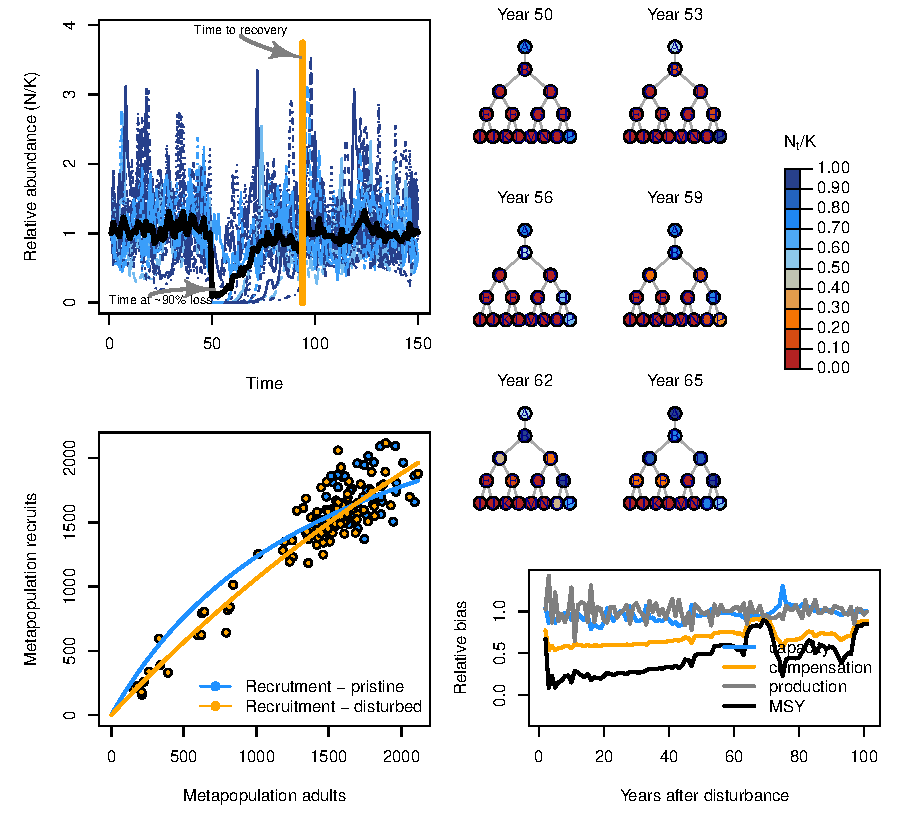
\includegraphics{Managing_for_ecological_surprises_in_metapopulations_makeHTML_files/figure-latex/example results4-1} 

}

\caption{Spatial recovery regime of stochastic metapopulation.}\label{fig:example results4}
\end{figure}

\hypertarget{simulation-test-bootstrap}{%
\subsection{Simulation test \&
bootstrap}\label{simulation-test-bootstrap}}

\hypertarget{general-patterns}{%
\subsubsection{General patterns}\label{general-patterns}}

We now show some general patterns in how variable patch demographic
rates, network structure, dispersal, disturbance, recruitment
stochasticity, and spatio-temporal correlations variation effects
metapopulation \emph{recovery rates}, \emph{maximum sustainable yield}
(i.e., analagous to the maximum rate of loss the system can sustain),
and \emph{coefficient of variation} across patches.

First, lets show recovery rates for a scenario where (1) patches have
the same local productivities, (2) patches have the same local carrying
capacities, (3) recruitment is deterministic, (4) there is no spatial
correlation in recruitment, and (5) there is no temporal correlations in
recruitment.

Below, we can see three main effects on recovery rates (number of
generations to reach recovery). First, recovery exponentially slows with
increased dispersal. Most of the action here takes place at low rates of
dispersal indicating most spatial topologies don't need much dispersal
to quicken their recovery. Second, more localized disturbances regimes
lead to slower recovery. Third, linearized networks have slower recovery
times than interconnected, complex networks suggesting that rescue
effects take some time to cascade through the entire network of patches.

\begin{figure}[H]

{\centering 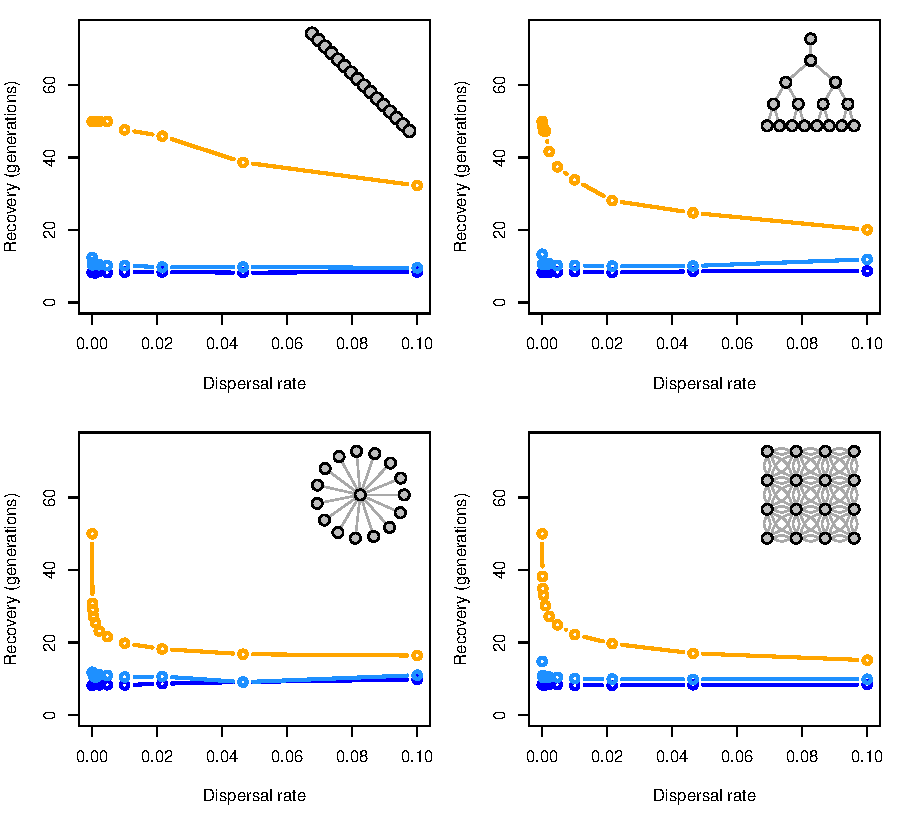
\includegraphics{Managing_for_ecological_surprises_in_metapopulations_makeHTML_files/figure-latex/general results-1} 

}

\caption{Recovery rates along dispersal, disturbance (blue - uniform; light blue - localized, random; orange - localized, extirpation), and network gradients without stochasticity.}\label{fig:general results}
\end{figure}

Now, lets show recovery rates for the same scenario with deterministic
recruitment but allowing for patches to vary in productivity and
carrying capacity. In addition to the same three main effects of
dispersal, network, and disturbance noted above, we also see variable
patch productivities substantially slows recovery times across all
scenarios.

\begin{figure}[H]

{\centering 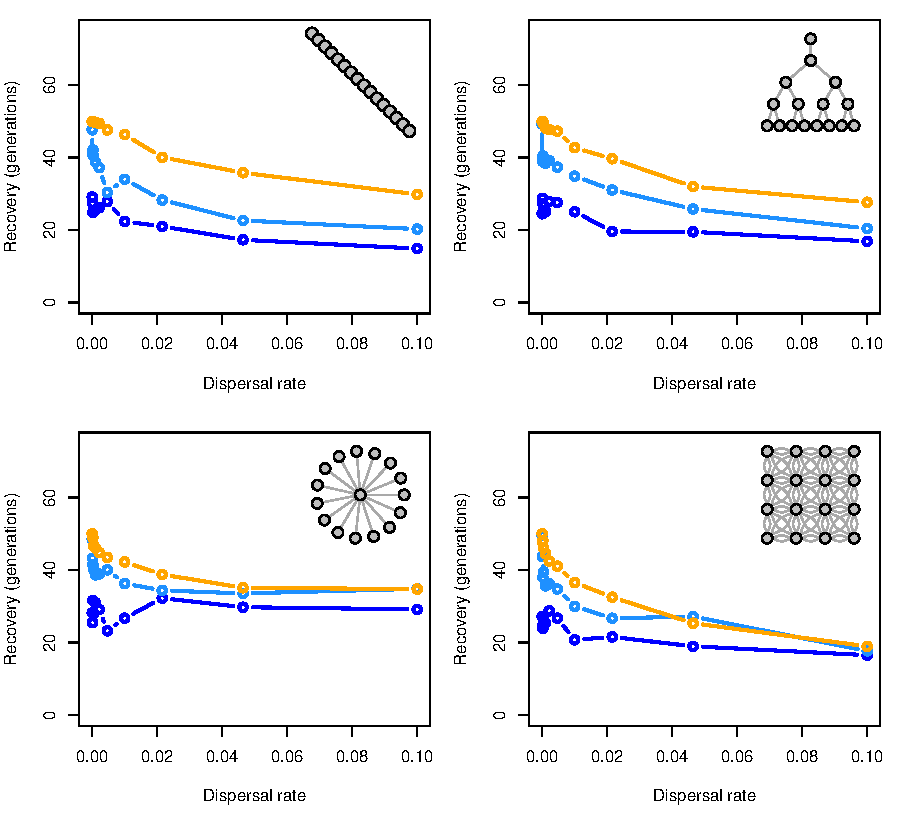
\includegraphics{Managing_for_ecological_surprises_in_metapopulations_makeHTML_files/figure-latex/results for variables patches-1} 

}

\caption{Recovery rates along dispersal, disturbance (blue - uniform; light blue - localized, random; orange - localized, extirpation), and network gradients with variable local productivity and carrying capacities.}\label{fig:results for variables patches}
\end{figure}

Now, lets show recovery rates for the same scenario but allowing for
recruitment to be stochastic (but patches are the same in demography).
We see the same three main effects of dispersal, network, and
disturbance noted above. We also see a few subtle changes: (1)
stochasticity slows recovery for uniform and local disturbance, but (2)
quickens recovery for extreme local disturbance.

\begin{figure}[H]

{\centering 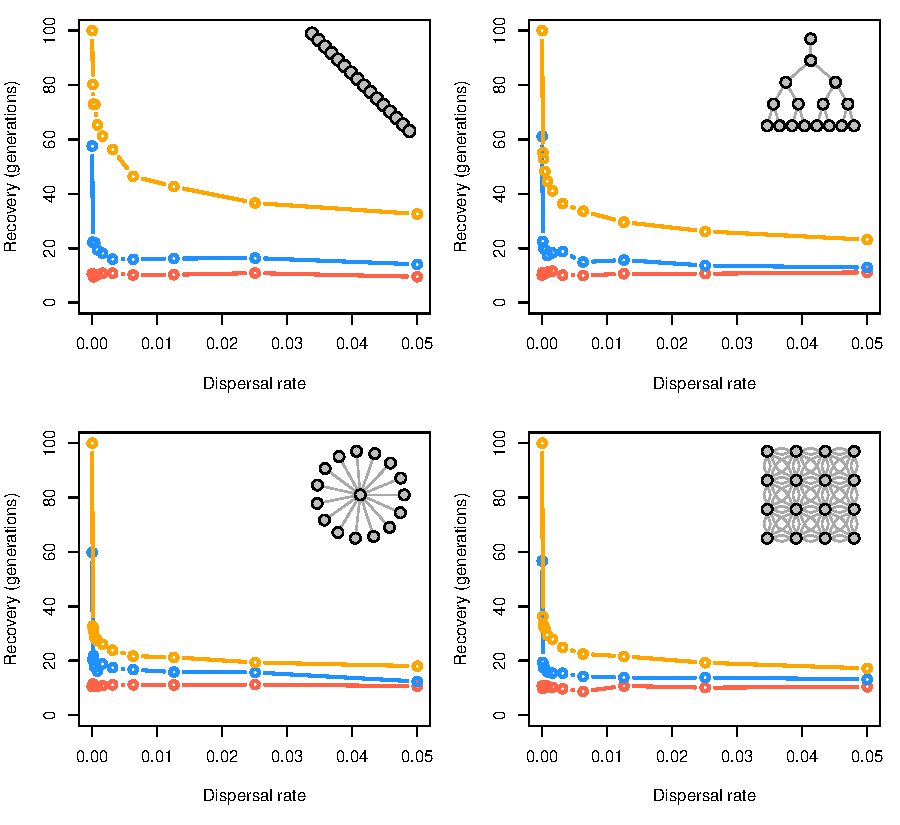
\includegraphics{Managing_for_ecological_surprises_in_metapopulations_makeHTML_files/figure-latex/stochastic recruitment-1} 

}

\caption{Recovery rates along dispersal, disturbance (blue - uniform; light blue - localized, random; orange - localized, extirpation), and network gradients with stochasticity.}\label{fig:stochastic recruitment}
\end{figure}

Now, lets show recovery rates for the same scenarios but with spatial
and temporal correlations in recruitment stochasticity. In addition to
the same effects of stochasticity, we also generally see a small effect
of slower recovery times for uniform and local disturbance, but faster
recovery times for extreme localized disturbance.

\begin{figure}[H]

{\centering 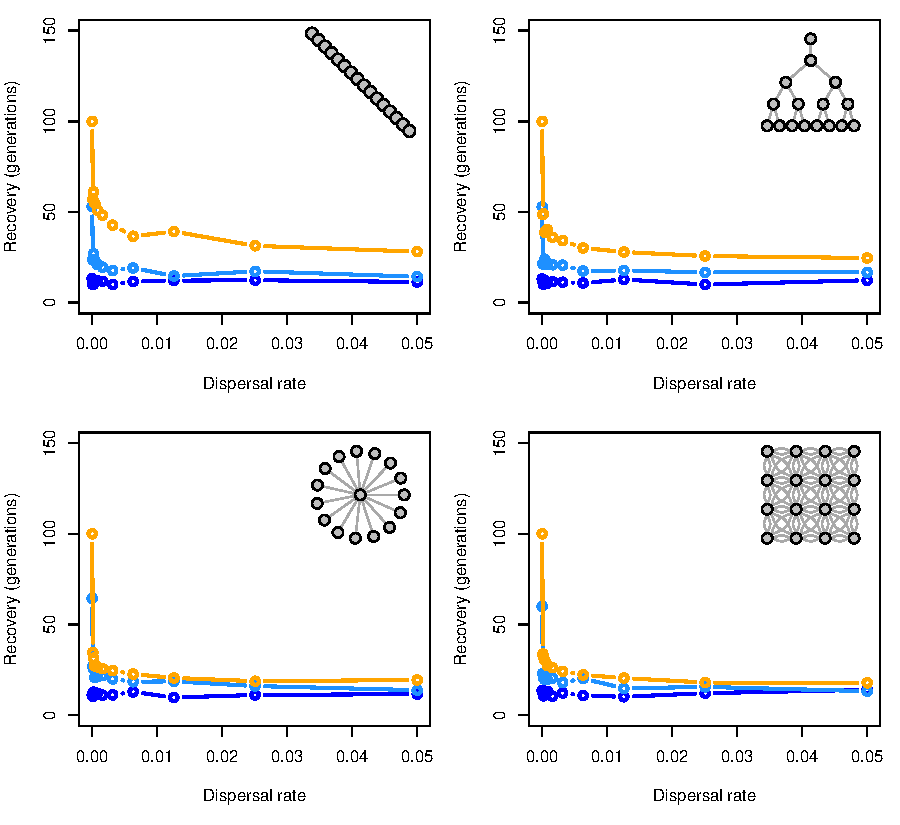
\includegraphics{Managing_for_ecological_surprises_in_metapopulations_makeHTML_files/figure-latex/spatiotemporal correlation-1} 

}

\caption{Recovery rates along dispersal, disturbance (blue - uniform; light blue - localized, random; orange - localized, extirpation), and network gradients with high spatial-temporal correlation in recruitment variation.}\label{fig:spatiotemporal correlation}
\end{figure}

\hypertarget{general-patterns-in-msy}{%
\paragraph{General patterns in MSY}\label{general-patterns-in-msy}}

\hypertarget{msy-with-deterministic-recruitment-where-patches-are-the-same}{%
\subparagraph{MSY with deterministic recruitment where patches are the
same}\label{msy-with-deterministic-recruitment-where-patches-are-the-same}}

We now show similar patterns in how maximum sustainable yield (MSY) of
the whole metapopulation shifts in the first 10 years post-disturbance
compared to the sum of MSY for each patch. A value of 1.0 would indicate
that the disturbed metapopulation can sustain itselfs against the same
disturbance regime as the sum of each patch independently. In other
words, is the metapopulation more, less, or equal to the sum of its
parts.

\begin{figure}[H]

{\centering 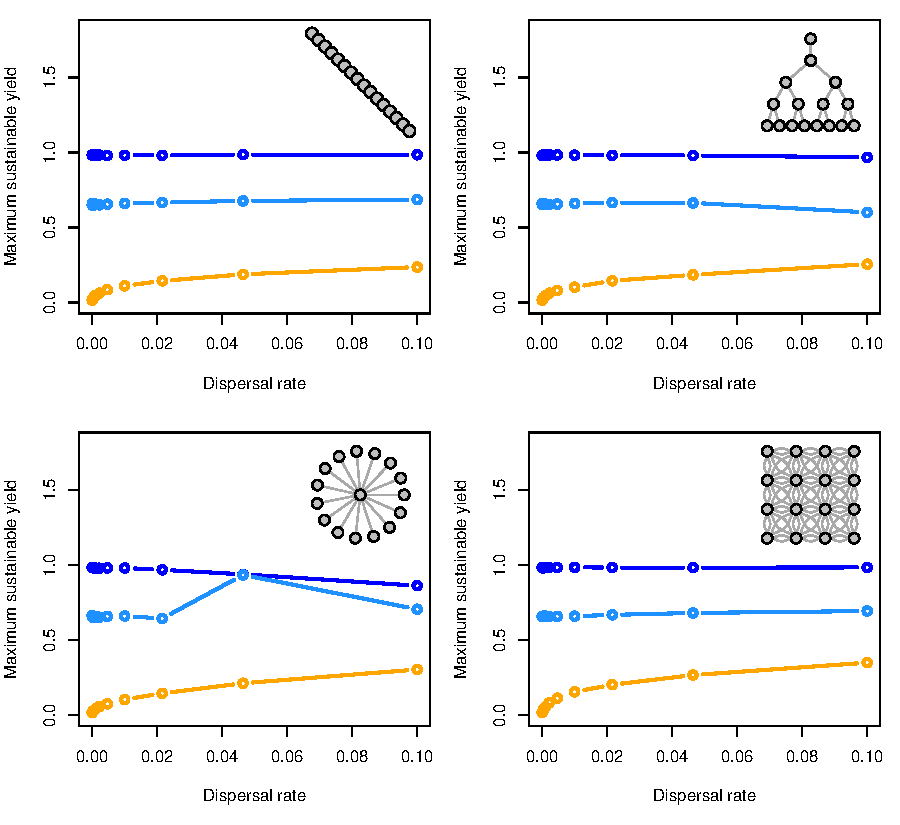
\includegraphics{Managing_for_ecological_surprises_in_metapopulations_makeHTML_files/figure-latex/MSY-1} 

}

\caption{Maximum sustainable yield along dispersal, disturbance (blue - uniform; light blue - localized, random; orange - localized, extirpation), and network gradients with high spatial-temporal correlation in recruitment variation.}\label{fig:MSY}
\end{figure}

\hypertarget{msy-with-variable-patches}{%
\subparagraph{MSY with variable
patches}\label{msy-with-variable-patches}}

Now, we illustrate how variable patch demography affects the 10-year
average MSY.

\begin{figure}[H]

{\centering 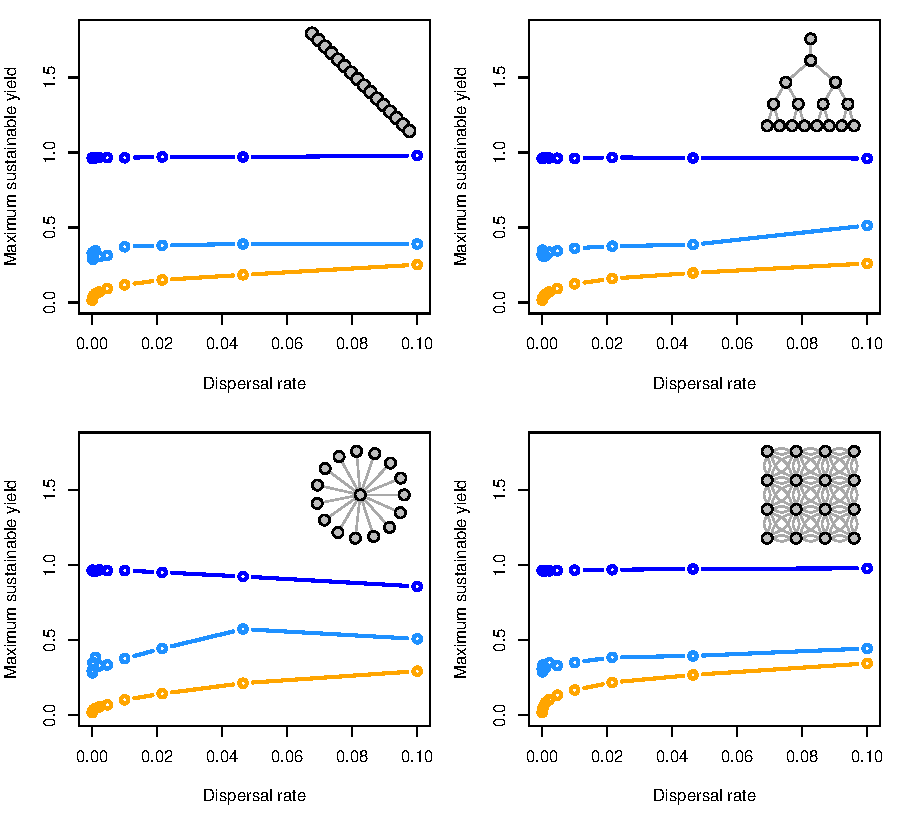
\includegraphics{Managing_for_ecological_surprises_in_metapopulations_makeHTML_files/figure-latex/MSY with variable patches-1} 

}

\caption{Maximum sustainable yield along dispersal, disturbance (blue - uniform; light blue - localized, random; orange - localized, extirpation), and network gradients with variable patches.}\label{fig:MSY with variable patches}
\end{figure}

\hypertarget{msy-with-variable-patches-and-stochasticity}{%
\subparagraph{MSY with variable patches and
stochasticity}\label{msy-with-variable-patches-and-stochasticity}}

Now, we illustrate how variable patch demography affects the 10-year
average MSY.

\begin{figure}[H]

{\centering 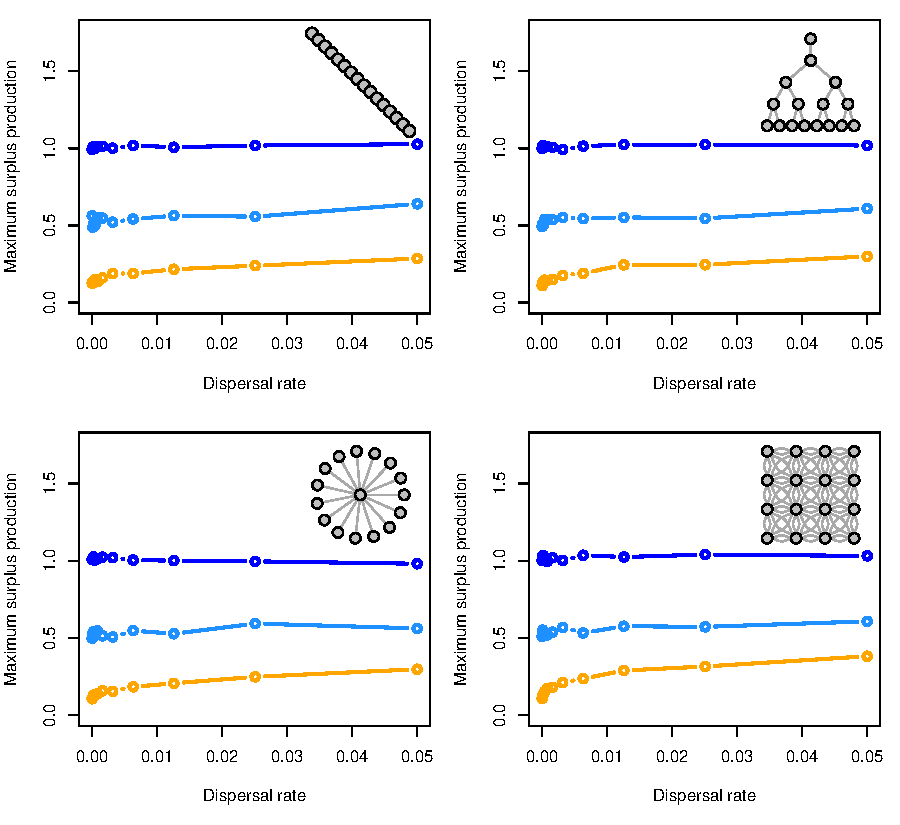
\includegraphics{Managing_for_ecological_surprises_in_metapopulations_makeHTML_files/figure-latex/MSY with variable patches and stochasticity-1} 

}

\caption{Maximum sustainable yield along dispersal, disturbance (blue - uniform; light blue - localized, random; orange - localized, extirpation), and network gradients with variable patches.}\label{fig:MSY with variable patches and stochasticity}
\end{figure}

\hypertarget{msy-with-variable-patches-and-spatio-temporally-correlated-stochasticity}{%
\subparagraph{MSY with variable patches, and spatio-temporally
correlated
stochasticity}\label{msy-with-variable-patches-and-spatio-temporally-correlated-stochasticity}}

Now, we illustrate how variable patch demography and high
spatial-temporal correlations in stochastic recrtuitment affects the
10-year average MSY.

\begin{figure}[H]

{\centering 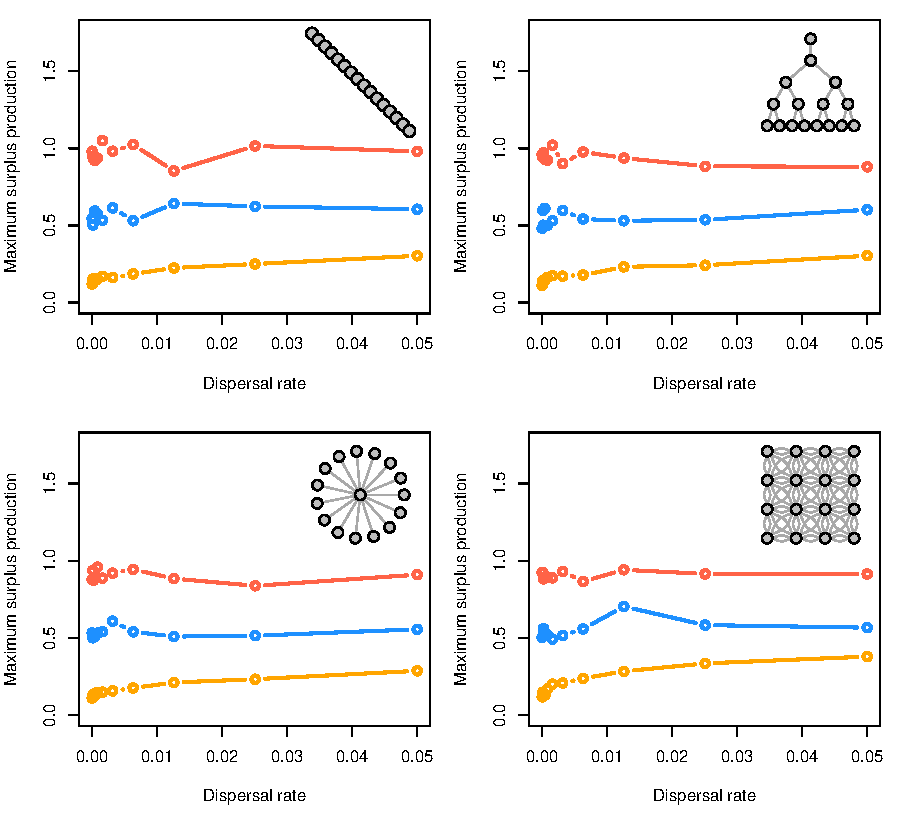
\includegraphics{Managing_for_ecological_surprises_in_metapopulations_makeHTML_files/figure-latex/MSY with variable patches and space-time stochasticity-1} 

}

\caption{Maximum sustainable yield along dispersal, disturbance (blue - uniform; light blue - localized, random; orange - localized, extirpation), and network gradients with variable patches.}\label{fig:MSY with variable patches and space-time stochasticity}
\end{figure}

\hypertarget{general-patterns-in-spatial-variation-across-patches}{%
\paragraph{General patterns in spatial variation across
patches}\label{general-patterns-in-spatial-variation-across-patches}}

\hypertarget{spatial-variation-with-deterministic-recruitment-where-patches-are-the-same}{%
\subparagraph{Spatial variation with deterministic recruitment where
patches are the
same}\label{spatial-variation-with-deterministic-recruitment-where-patches-are-the-same}}

We now show similar patterns in how the coefficient of variation (CV)
across all patches within the metapopulation shifts in the first 10
years post-disturbance.

\begin{figure}[H]

{\centering 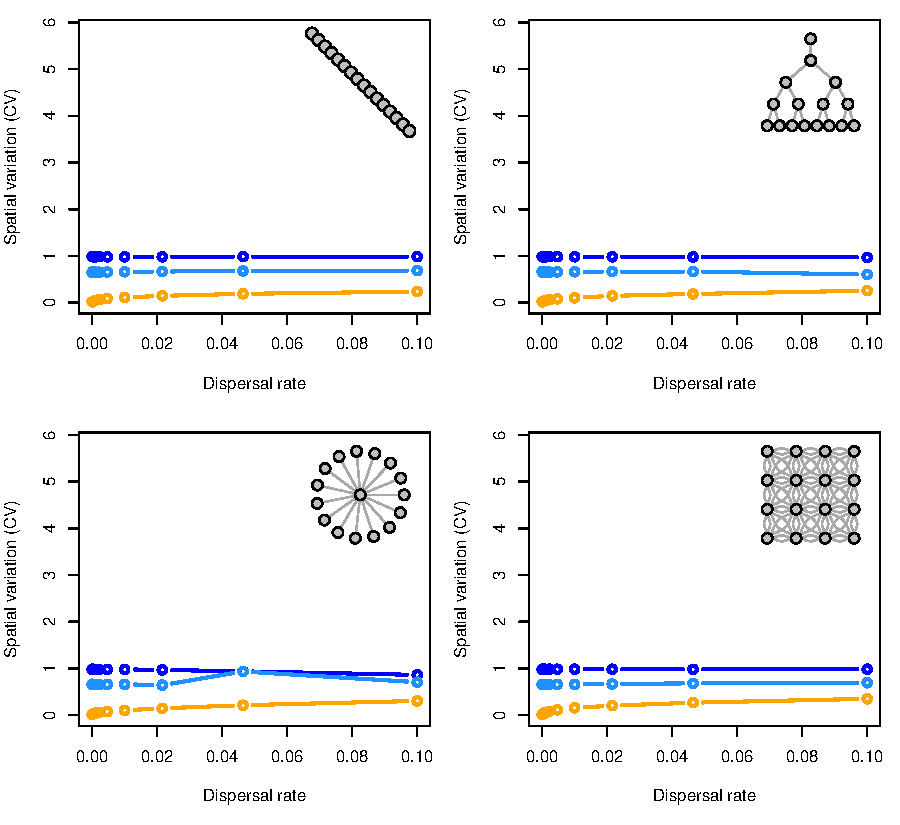
\includegraphics{Managing_for_ecological_surprises_in_metapopulations_makeHTML_files/figure-latex/CV-1} 

}

\caption{Maximum sustainable yield along dispersal, disturbance (blue - uniform; light blue - localized, random; orange - localized, extirpation), and network gradients with high spatial-temporal correlation in recruitment variation.}\label{fig:CV}
\end{figure}

\hypertarget{spatial-variation-with-variable-patches}{%
\subparagraph{Spatial variation with variable
patches}\label{spatial-variation-with-variable-patches}}

Now, we illustrate how variable patch demography affects the 10-year
average CV.

\begin{figure}[H]

{\centering 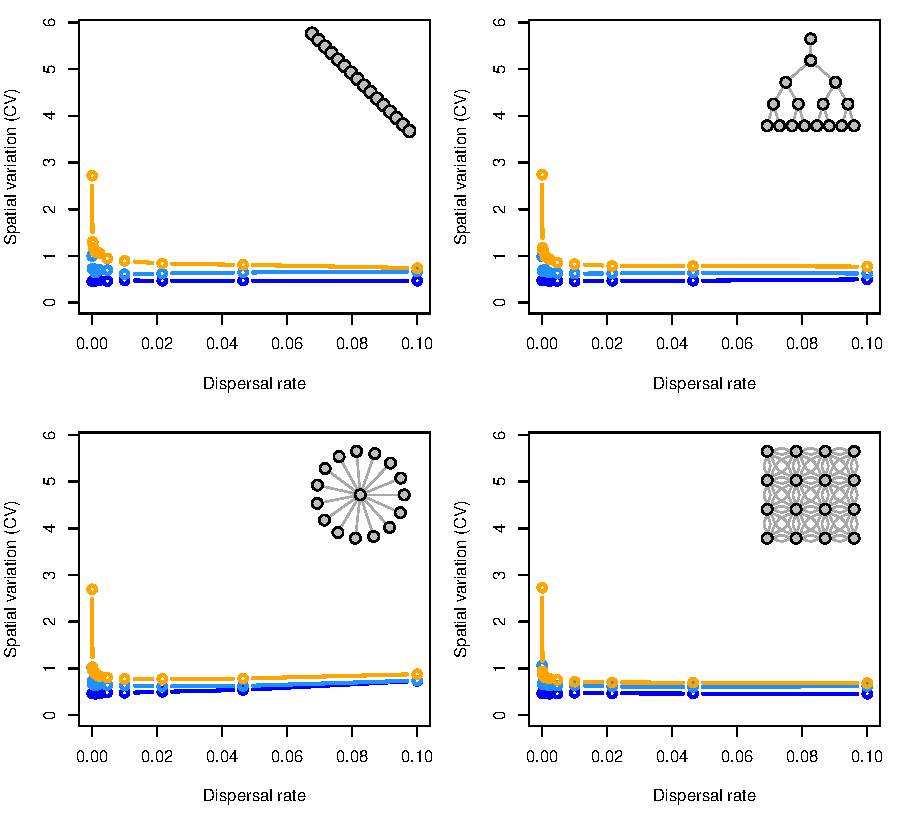
\includegraphics{Managing_for_ecological_surprises_in_metapopulations_makeHTML_files/figure-latex/CV with variable patches-1} 

}

\caption{Spatial variation along dispersal, disturbance (blue - uniform; light blue - localized, random; orange - localized, extirpation), and network gradients with variable patches.}\label{fig:CV with variable patches}
\end{figure}

\hypertarget{spatial-variation-with-variable-patches-and-stochasticity}{%
\subparagraph{Spatial variation with variable patches and
stochasticity}\label{spatial-variation-with-variable-patches-and-stochasticity}}

Now, we illustrate how variable patch demography affects the 10-year
average CV.

\begin{figure}[H]

{\centering 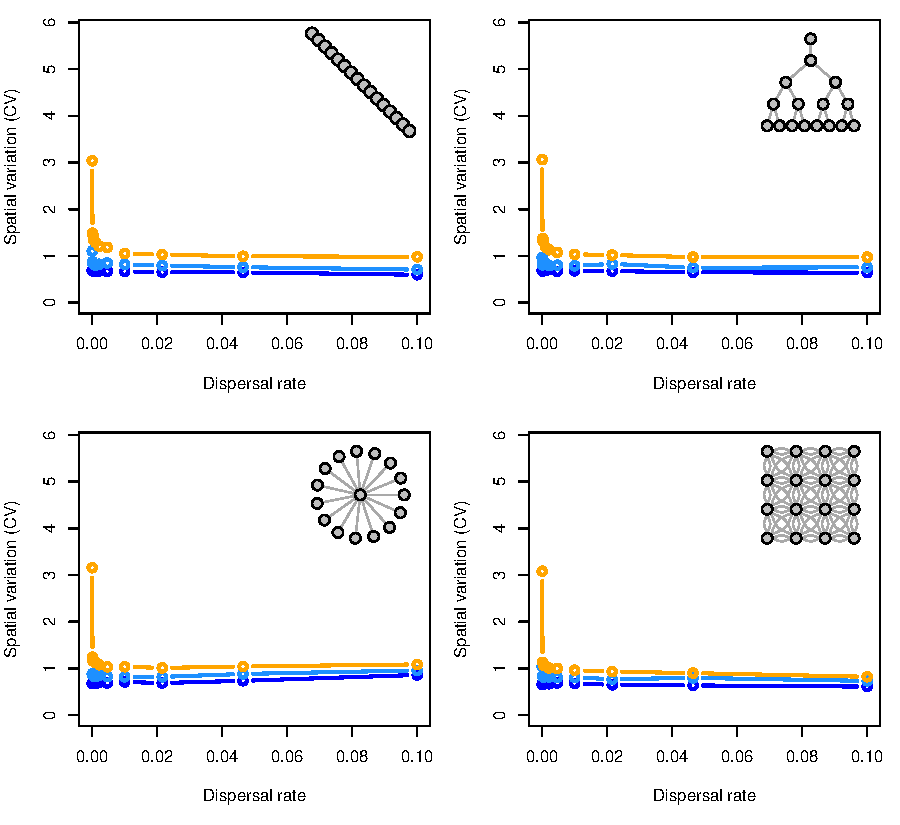
\includegraphics{Managing_for_ecological_surprises_in_metapopulations_makeHTML_files/figure-latex/CV with variable patches and stochasticity-1} 

}

\caption{Spatial variation along dispersal, disturbance (blue - uniform; light blue - localized, random; orange - localized, extirpation), and network gradients with variable patches and stochastic recruitment.}\label{fig:CV with variable patches and stochasticity}
\end{figure}

\hypertarget{spatial-variation-with-variable-patches-and-spatio-temporally-correlated-stochasticity}{%
\subparagraph{Spatial variation with variable patches, and
spatio-temporally correlated
stochasticity}\label{spatial-variation-with-variable-patches-and-spatio-temporally-correlated-stochasticity}}

Now, we illustrate how variable patch demography and high
spatial-temporal correlations in stochastic recrtuitment affects the
10-year average CV.

\begin{figure}[H]

{\centering 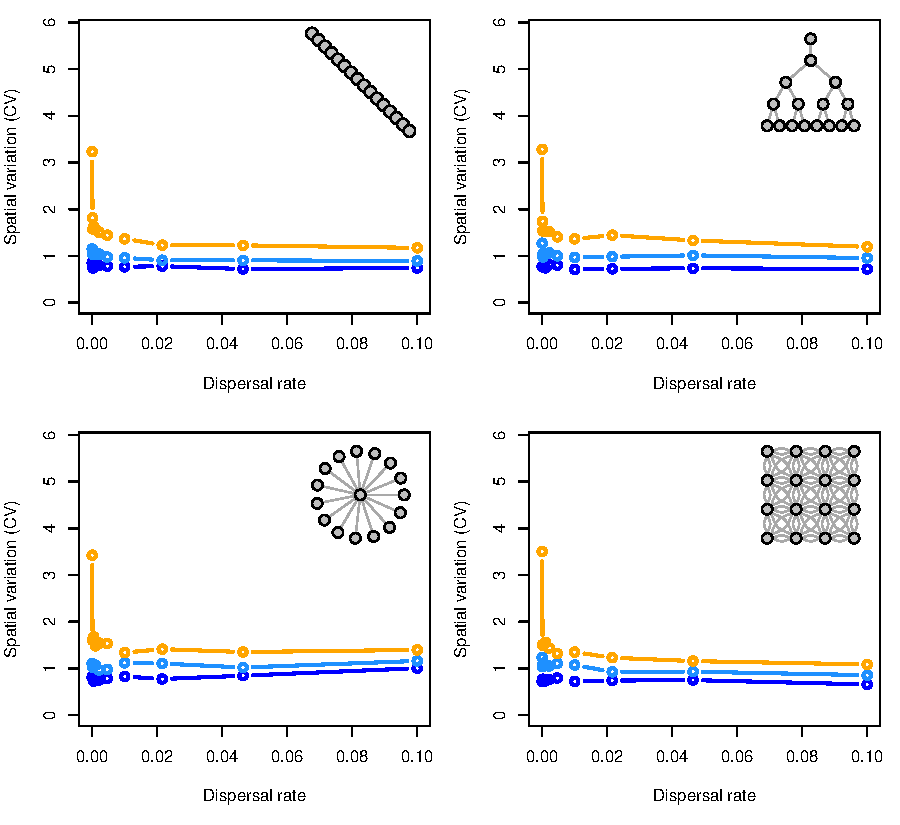
\includegraphics{Managing_for_ecological_surprises_in_metapopulations_makeHTML_files/figure-latex/CV with variable patches and space-time stochasticity-1} 

}

\caption{Spatial variation along dispersal, disturbance (blue - uniform; light blue - localized, random; orange - localized, extirpation), and network gradients with variable patches, and spatial-temporal correlations in stochastic recruitment.}\label{fig:CV with variable patches and space-time stochasticity}
\end{figure}


\end{document}
